\section{Bayes' Theorem}
There are two different philosophies in statistics: the Frequentist and Bayesian. Most of the statistical formulation in this dissertation is made in Bayesian statistics, so this will be the one explained and focused.

\begin{equation}
    \label{eq: bayes theorem}
    P(H|E) = \frac{P(H) \times P(E|H)}{P(E)}
\end{equation}

Bayes' theorem (equation \ref*{eq: bayes theorem}) gives the probability of some hypothesis $H$ happening knowing that the event $E$ has ocorred. $P(H)$, also known as the \textit{prior} probability, states the probability of the hypothesis $H$ to be true. $P(E|H)$ is the probability of the event happening given the hypothesis is true and $P(E)$ is the probability of the event occurring. Bayes' theorem essentially tells how to update our beliefs in the light of new evidence, but it does not state how to set up our \textit{prior} beliefs. The idea is to keep updating our beliefs to increase the amount of confidence they are indeed correct. Therefor, this formulation is not designed to be used a single time, it is designed to be used in multiple iterations. The initial \textit{prior} probability is usually a guess and in the following iterations is many times considered to be equal to the previous iteration $P(H|E)$, also known as the \textit{posterior} probablity. In each iteration the probability of the hypothesis $P(H|E)$ to be true is updated based on new information received and the new \textit{prior} probability.  where the \textit{prior} probability is a guess and in each iteration the probability of the hypothesis $H$ is updated, where the \textit{prior} probability can be equal to the previous iteration $P(H|E)$, known as a \textit{posterior} probability, based on new information received. A common assumption to make is that every iteration is independent of the previous one, this is known as the Markov assumption:

\begin{equation}
    P(X_n = x_n | X_{n-1} = x_{n-1}, ..., X_0 = x_0) = P(X_n = x_n | X_{n-1} = x_{n-1})
\end{equation}

\section{Gaussian random variables}
Every sensor measure is noisy, so each measurement has an associated uncertainty. The measurement given by the sensor are therefor considered to be random variables. The \acl*{PDF} (\acs*{PDF}) is a function that provides the probability of a random variable to be within a specific interval of values. Many times, the noises envolved in measurements follows a Gaussian or Normal distribution, which have the equation \ref*{eq: gaussian pdf} and takes the form of Figure \ref*{fig: normal pdf}.

\begin{equation}
    \label{eq: gaussian pdf}
    g(x) = \frac{1}{\sigma\sqrt{2\pi}}\exp(-\frac{1}{2}\times\frac{(x - \mu)^2}{\sigma^2})
\end{equation}

\begin{figure}[H]
    \centering
    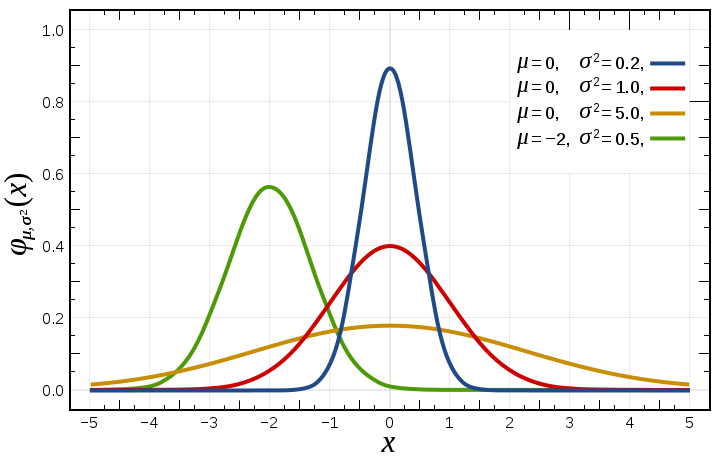
\includegraphics[width=0.5\linewidth]{images/statistics/Normal_Distribution_PDF.png}
    \caption{Normalized Gaussian curves with expected value $\mu$ and variance $\sigma^2$ \cite{enwiki:1100476982}}
    \label{fig: normal pdf}
\end{figure}

An interesting property of a Gaussian random variables is that they can be passed through a linear function and the output will also result in a gaussian random variable,, with a different mean and \acs*{STD}. This property \textbf{only holds} for linear functions. One has two different ways to solve the problem for passing a random variable through a nonlinear function. The first is to locally linearize with the first order Taylor Expansion Series:

\begin{equation}
    T(x) = \sum_{n=0}^{\infty} \frac{f^{(n)}(a)}{n!}(x-a)^n
\end{equation}

\todo[inline]{Insert image of a function and Taylor Expansion}

This will make the function locally linear, but not every function will be well represented with a first order expansion. Other problem is that to compute the first Taylor expansion, one must perform heavy calculate calculations, which makes the process slow.
The other method is to pass several values of the initial random variable through the nonlinear function, for instance, consider the nonlinear function:

\begin{equation}
    y(x) = 3x^3 + 2x^2 + x
\end{equation}

and we can compute $y(\mu)$, $y(\mu+\sigma)$, $y(\mu-\sigma)$, $y(\mu+2\sigma)$, $y(\mu-2\sigma)$, etc... if the considered $x$ values are around the mean we can compute the mean and \acs*{STD} of the y from these values. This will make $y$ a gaussian random variable. This is called an \textbf{Unscented Transform}


\section{Kalman Filters}

\todo[inline]{Explain assumptions needed}

\todo[inline]{Explain the workflow of the algorithm}

\section{Particle Filters}